%%%%%%%%%%%%%%%%%%%%%%%%%%%%%%%%%%%%%%%%%%%%%%%%%%%
%
%  New template code for TAMU Theses and Dissertations starting Fall 2012.  
%  For more info about this template or the 
%  TAMU LaTeX User's Group, see http://www.howdy.me/.
%
%  Author: Wendy Lynn Turner 
%	 Version 1.0 
%  Last updated 8/5/2012
%
%%%%%%%%%%%%%%%%%%%%%%%%%%%%%%%%%%%%%%%%%%%%%%%%%%%
%%%%%%%%%%%%%%%%%%%%%%%%%%%%%%%%%%%%%%%%%%%%%%%%%%%%%%%%%%%%%%%%%%%%%%
%%                           SECTION V
%%%%%%%%%%%%%%%%%%%%%%%%%%%%%%%%%%%%%%%%%%%%%%%%%%%%%%%%%%%%%%%%%%%%%


\chapter{\uppercase{Experiments, Results and Analysis}}

In this chapter, I will highlight and analyze the training process and the results for each of the components of our model. 

\section{Dataset Processing}

YOLO needs certain specific files to know how and what to train. As DeepFlow is based on this object detection framework, we must create some configuration files and place them in a configuration folder, named cfg, that will be accessed by our application at the time of training as well as testing. These files are: \textbf{obj.data} which contains the training and text labels in a .txt format,\textbf{obj.names} which containes the different object categories that will be used to identify objects, and \textbf{yolo-obj2.cfg} which contains all the parameters needed for training such as number of batches, number of object categories, number of iterations, learning rate as well as settings for training the network with a gpu or cpu, etc.  The batch size was related to the grid size of the model, with a learning rate of 0.001. In order to reduce the memory footprint and increase computational efficiency of our model, just like in YOLO, all images are first resized to 416 x 416 pixels at both training and testing times. 

\vspace{15mm}
\newpage
Figure \ref{cfg_file} shows how our configuration files looks:

\vspace{15mm}
\begin{figure}[h]
\centering
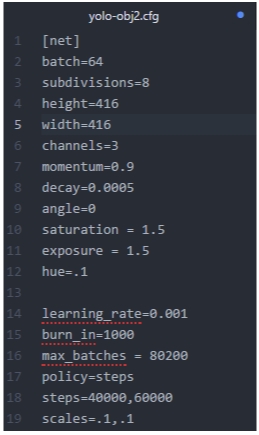
\includegraphics[scale=0.87]{figures/cfg_file.png}
\caption{YOLO Configuration file}
\label{cfg_file}
\end{figure}

\newpage
\section{Dataset Training and Testing Results}
\vspace{5mm}
The entire training log below represents one batch of images, divided according to our subdivisions. We can see the .cfg file shown earlier in Figure \ref{cfg_file} to verify that batch = 64 and subdivision = 8. Looking at the image above, the training iteration has 8 groups of 8 images, reflecting these specific settings.

\vspace{5mm}
\begin{lstlisting}
Loaded: 5.588888 seconds
Region Avg IOU: 0.649881, Class: 0.854394, Obj: 0.476559, No Obj: 0.007302, Avg Recall: 0.737705,  count: 61
Region Avg IOU: 0.671544, Class: 0.959081, Obj: 0.523326, No Obj: 0.006902, Avg Recall: 0.780000,  count: 50
Region Avg IOU: 0.525841, Class: 0.815314, Obj: 0.449031, No Obj: 0.006602, Avg Recall: 0.484375,  count: 64
Region Avg IOU: 0.583596, Class: 0.830763, Obj: 0.377681, No Obj: 0.007916, Avg Recall: 0.629214,  count: 89
Region Avg IOU: 0.651377, Class: 0.908635, Obj: 0.460094, No Obj: 0.008060, Avg Recall: 0.753425,  count: 73
Region Avg IOU: 0.571363, Class: 0.880554, Obj: 0.341659, No Obj: 0.007820, Avg Recall: 0.633663,  count: 101
Region Avg IOU: 0.585424, Class: 0.935552, Obj: 0.358635, No Obj: 0.008192, Avg Recall: 0.644860,  count: 107
Region Avg IOU: 0.599972, Class: 0.832793, Obj: 0.382910, No Obj: 0.009005, Avg Recall: 0.650602,  count: 83
497001: 0.863348, 0.863348 avg, 0.000012 rate, 5.422251 seconds, 107352216 images
\end{lstlisting}

\vspace{5mm}
As we can see in the above listing the last line shows what the batch output is at the moment of training:
\begin{enumerate}
  \item Training batch: 497001.
  \item Total loss:0.863348.
  \item Average loss error: 0.863348 avg, which should be as low as possible in order for us to stopped training the network.
  \item Learning rate that we specified in the configuration file.
  \item Time spent to process the image batch and the total amount of images used during training at this point 5.422251 for 107352216 images.
\end{enumerate}

\vspace{5mm}
The following code snippet illustrates how we log the above training process. By doing this, we are allow the chance to improve our model so that it can be trained in a more efficient way thus delivering better performance in our final application:

\vspace{5mm}
\begin{lstlisting}
def extract_log(log_file,new_log_file,key_word):

    f = open(log_file)
    train_log = open(new_log_file, 'w')

    for line in f:
        if 'Syncing' in line:
            continue
        # Remove the log with zero error
        if 'nan' in line:
            continue
        if key_word in line:
            train_log.write(line)

    f.close()
    train_log.close()

extract_log('coco_train_log.txt','coco_train_log_loss.txt','images')
extract_log ( ' coco_train_log.txt ' , ' coco_train_log_iou.txt ' , ' IOU ' )
\end{lstlisting}

\vspace{5mm}
In our re-implementation of DeepFlow, a YOLO object detection and tracking system, we have initially used PASCAL-VOC for faster training and testing of our system. Nonetheless, this dataset has a limitation for our application since it only offers a limited number of categories, 20 classes and our mindset is for our application to be able to identify and track at least 80 to 100 object categories. Therefore, we decided for our final application to use COCO DATASET which is a large-scale object detection, segmentation, and captioning dataset with several advantages for research in the field of computer vision. The dataset offers 330k+ images, recognition in context, 80 object categories, and many other features that we will use for our advantage to train and test our network.

\newpage
When using PASCAL-VOC which is a lighter dataset that can be easily trained and test in a few hours on a laptop since it needs less training steps than other datasets such as COCO,PASCAL-VOC comes almost pre-trained from ImageNet. Therefore, the training scope boils down only to adding specific layers for new recognition tasks by using the previous learned knowledge.

Figure \ref{test_graph} shows the statistics of our training using PASCAL-VOC:
\begin{figure}[h]
\centering
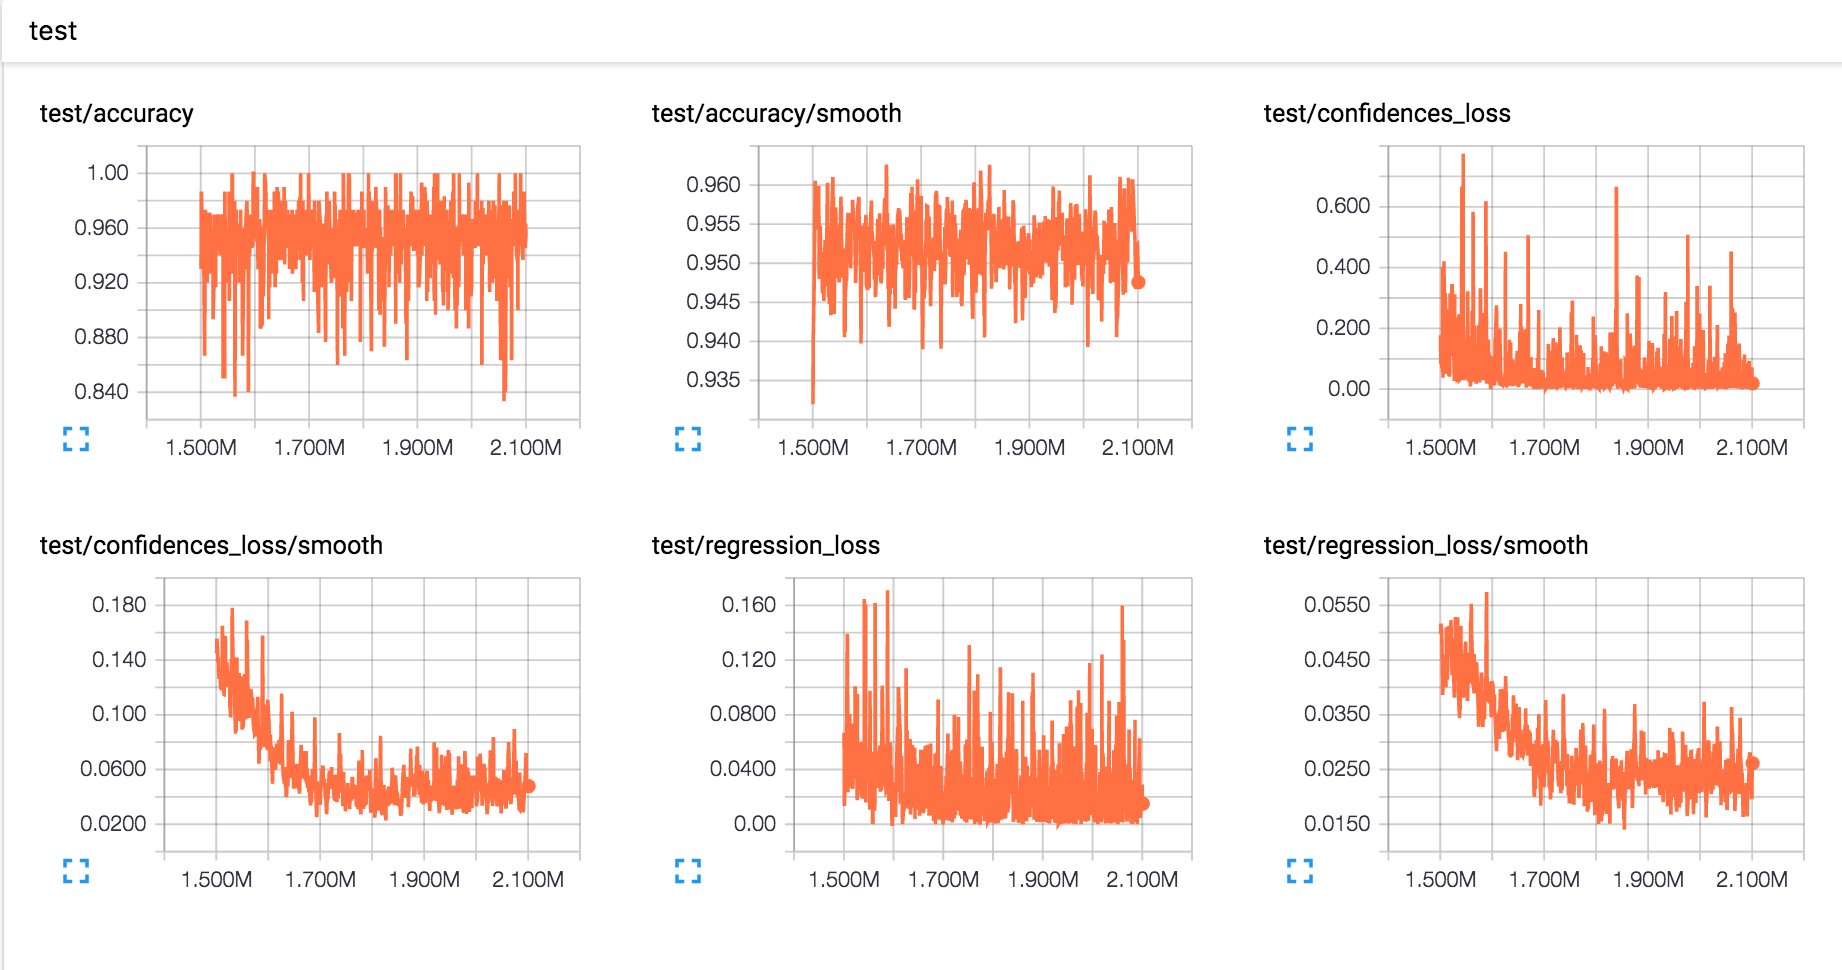
\includegraphics[scale=0.2]{figures/test_graph.png}
\caption{PASCAL-VOC Training Graph}
\label{test_graph}
\end{figure}

As we can see in training accuracy and cross-entropy cost function graphs both functions flatten due our model only focusing on 20 - 30  classes of a few  objects it already knows. Figures \ref{accuracy_crossentropy} below highlights that the graph learns well.

\begin{figure}
\centering
\begin{subfigure}{.5\textwidth}
  \centering
  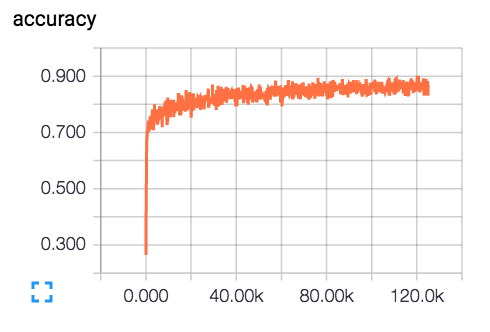
\includegraphics[width=.8\linewidth]{figures/graph_accuracy.png}
  \caption{Training Accuracy}
  \label{fig:sub1}
\end{subfigure}%
\begin{subfigure}{.5\textwidth}
  \centering
  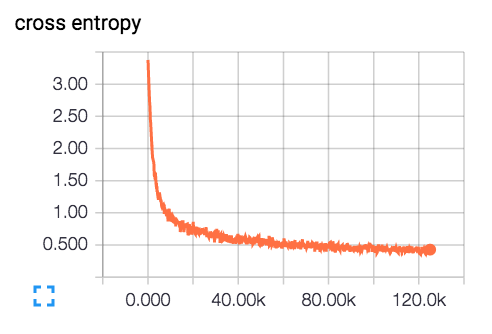
\includegraphics[width=.8\linewidth]{figures/cross_entropy.png}
  \caption{Cross Entropy Cost Function}
  \label{fig:sub2}
\end{subfigure}
\caption{Traing Accuracy and Cross Entropy Cost Function}
\label{fig:accuracy_crossentropy}
\end{figure}

\newpage
for our final application in order to achieve an acceptable performance comparable to YOLO using a larger dataset like COCO, we had to train our network for a couple of days. Initially, we got not so good results due to the fact that our implementation performance was too slow to learn. Learning was inaccurate leading to bad performance while using both GPU and CPU. 

In order to improve performance, we decided to use Tensorbox to help in the training process. As we can see from the graphs in figure \ref{training_graph_tf}, all functions flatten with sparse results and peaks. This happens because of generalization of the model which is not learning different masks for each object category which reduces our accuracy while training.


\begin{figure}[h]
\centering
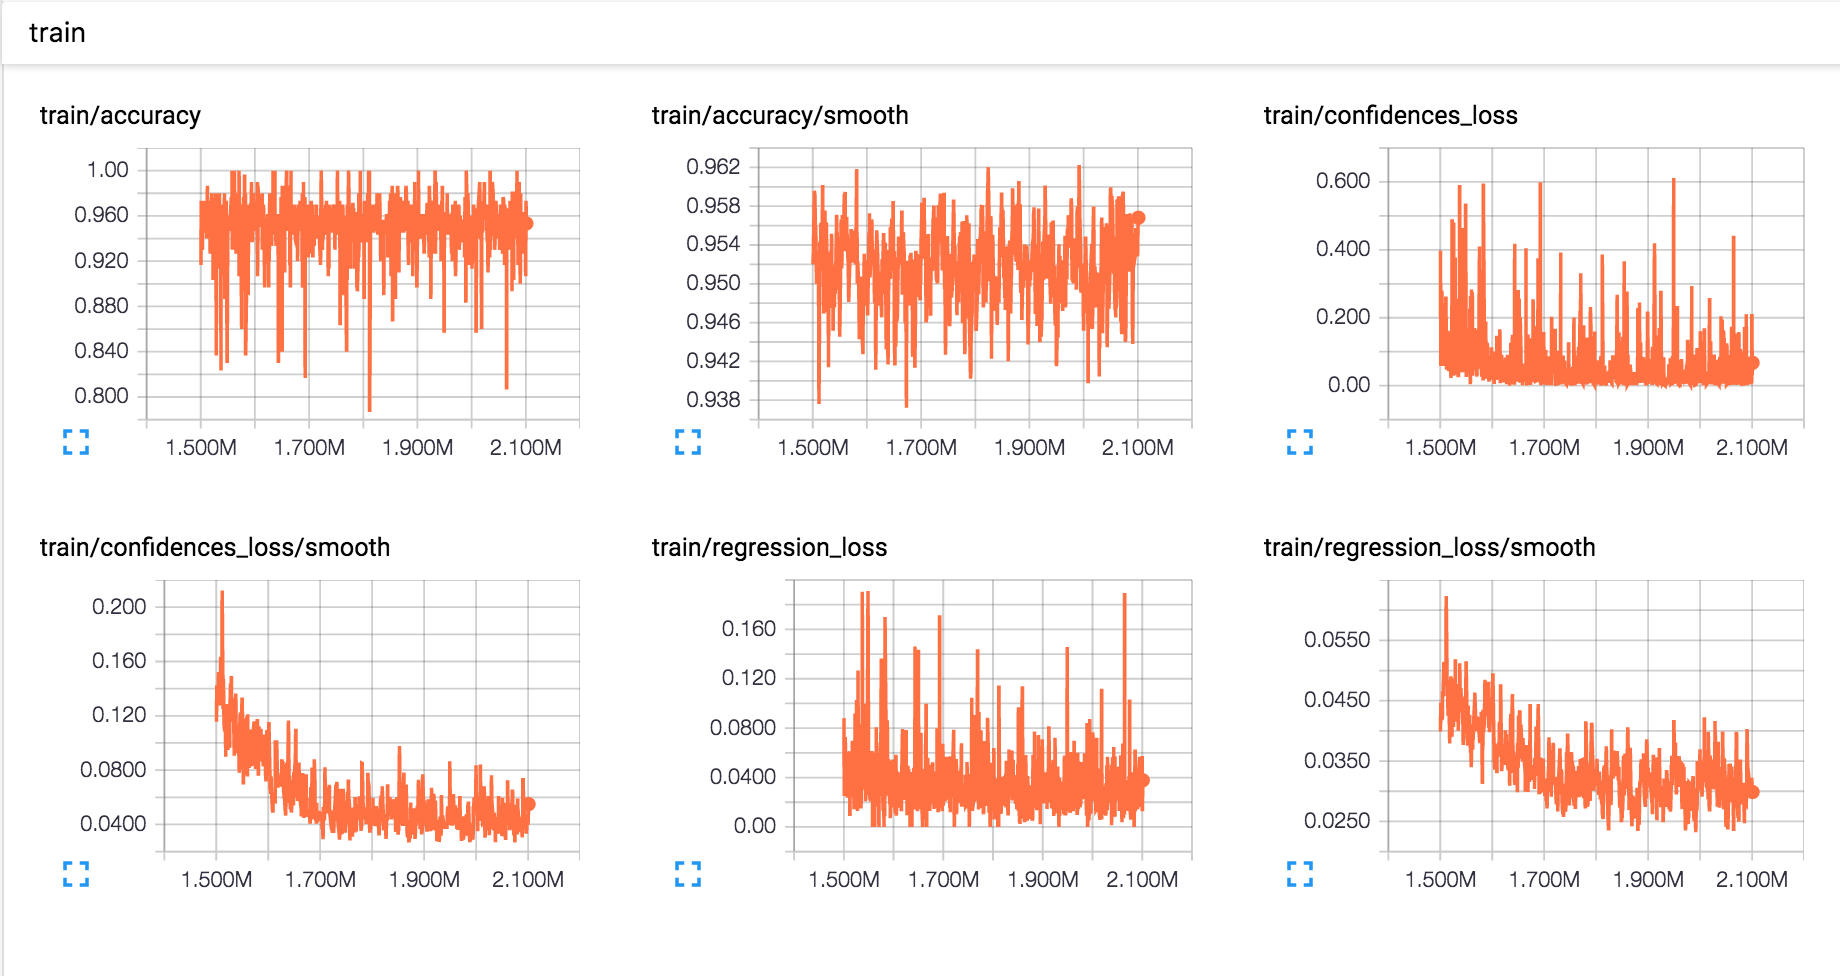
\includegraphics[scale=0.3]{figures/training_graph_tf.png}
\caption{DeepFlow Configuration file}
\label{training_graph_tf}
\end{figure}

\newpage
As figure \ref{weights_norm} shows that the weights of our model, after some iterations, flatten what let us know that the model was not learning any more.

\begin{figure}[h]
\centering
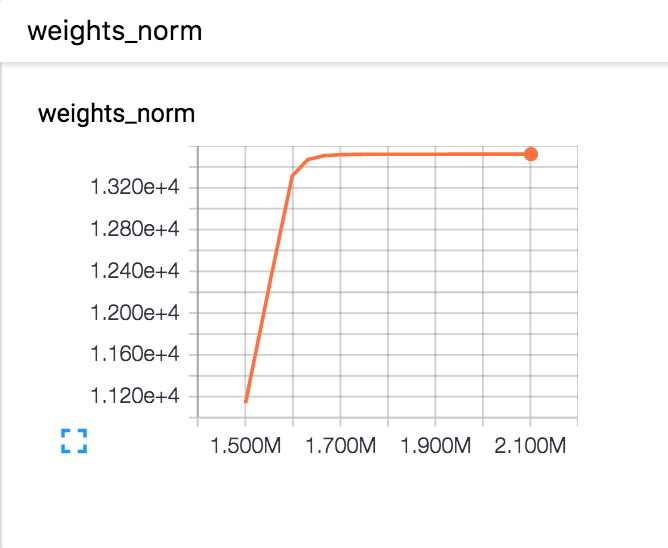
\includegraphics[scale=0.3]{figures/weights_norm.png}
\caption{Weights from first training results}
\label{weights_norm}
\end{figure}

Below, we show some screenshots of our first tests of the exported model where we have some degree of  inaccuracy when detecting objects:

\begin{figure}
\centering
\begin{subfigure}{.5\textwidth}
  \centering
  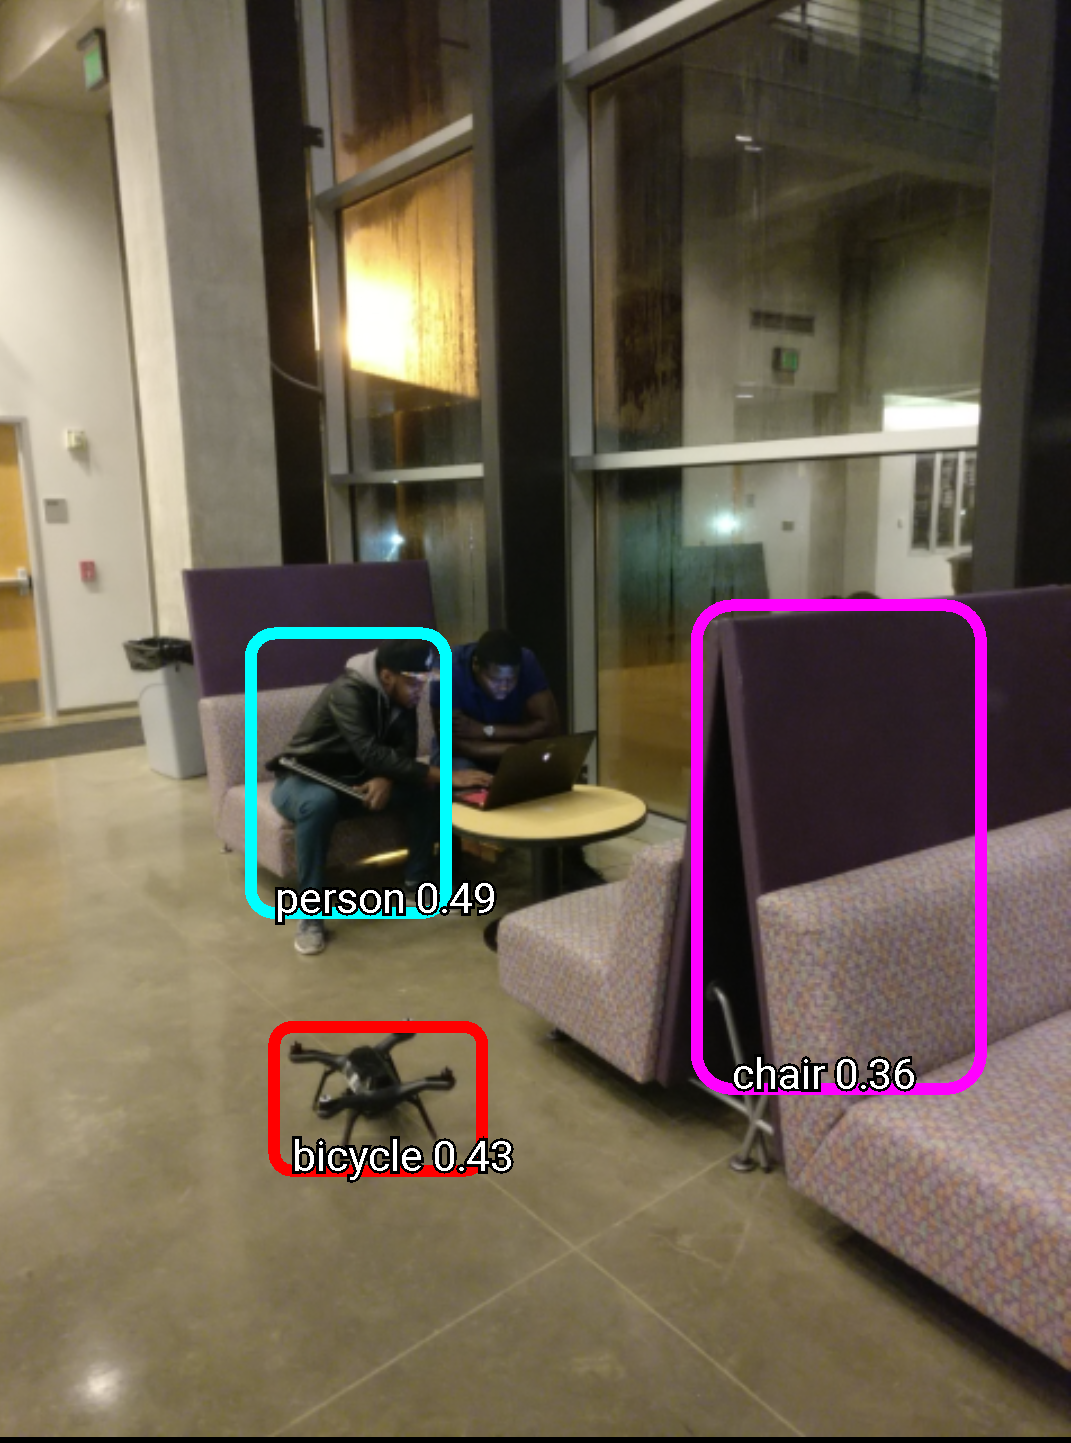
\includegraphics[width=.4\linewidth]{figures/test_2.png}
  \caption{Detection Accuracy Test}
  \label{fig:sub1}
\end{subfigure}%
\begin{subfigure}{.5\textwidth}
  \centering
  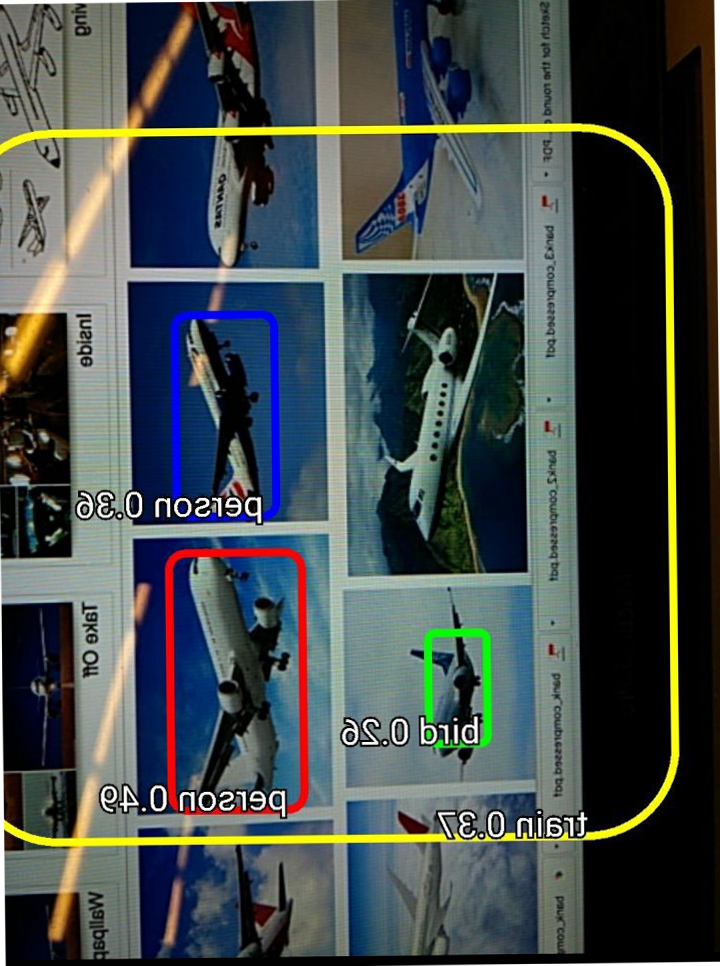
\includegraphics[width=.4\linewidth]{figures/test_7.png}
  \caption{Detection Accuracy Test}
  \label{fig:sub2}
\end{subfigure}
\caption{DeepFlow Object Detection Accuracy Test}
\label{fig:accuracy_test}
\end{figure}

\newpage
Due to  bad results obtained in the first days of training, we upgraded our network to improve training and thus, obtaining better learning rates as well as better detection and tracking results.

The code implementation for training below shows our modified network and the graph output:

\vspace{3mm}
\begin{lstlisting}
import os
import argparse
import configparser
import importlib
import shutil
import time
import inspect
import multiprocessing
import tensorflow as tf
import tensorflow.contrib.slim as slim
import utils.data


def summary_scalar(config):
    try:
        reduce = eval(config.get('summary', 'scalar_reduce'))
        for t in utils.match_tensor(config.get('summary', 'scalar')):
            name = t.op.name
            if len(t.get_shape()) > 0:
                t = reduce(t)
                tf.logging.warn(name + ' is not a scalar tensor, reducing by ' + reduce.__name__)
            tf.summary.scalar(name, t)
    except (configparser.NoSectionError, configparser.NoOptionError):
        tf.logging.warn(inspect.stack()[0][3] + ' disabled')


def summary_image(config):
    try:
        for t in utils.match_tensor(config.get('summary', 'image')):
            name = t.op.name
            channels = t.get_shape()[-1].value
            if channels not in (1, 3, 4):
                t = tf.expand_dims(tf.reduce_sum(t, -1), -1)
            tf.summary.image(name, t, config.getint('summary', 'image_max'))
    except (configparser.NoSectionError, configparser.NoOptionError):
        tf.logging.warn(inspect.stack()[0][3] + ' disabled')


def summary_histogram(config):
    try:
        for t in utils.match_tensor(config.get('summary', 'histogram')):
            tf.summary.histogram(t.op.name, t)
    except (configparser.NoSectionError, configparser.NoOptionError):
        tf.logging.warn(inspect.stack()[0][3] + ' disabled')


def summary(config):
    summary_scalar(config)
    summary_image(config)
    summary_histogram(config)


def get_optimizer(config, name):
    section = 'optimizer_' + name
    return {
        'adam': lambda learning_rate: tf.train.AdamOptimizer(learning_rate, config.getfloat(section, 'beta1'), config.getfloat(section, 'beta2'), config.getfloat(section, 'epsilon')),
        'adadelta': lambda learning_rate: tf.train.AdadeltaOptimizer(learning_rate, config.getfloat(section, 'rho'), config.getfloat(section, 'epsilon')),
        'adagrad': lambda learning_rate: tf.train.AdagradOptimizer(learning_rate, config.getfloat(section, 'initial_accumulator_value')),
        'momentum': lambda learning_rate: tf.train.MomentumOptimizer(learning_rate, config.getfloat(section, 'momentum')),
        'rmsprop': lambda learning_rate: tf.train.RMSPropOptimizer(learning_rate, config.getfloat(section, 'decay'), config.getfloat(section, 'momentum'), config.getfloat(section, 'epsilon')),
        'ftrl': lambda learning_rate: tf.train.FtrlOptimizer(learning_rate, config.getfloat(section, 'learning_rate_power'), config.getfloat(section, 'initial_accumulator_value'), config.getfloat(section, 'l1_regularization_strength'), config.getfloat(section, 'l2_regularization_strength')),
        'gd': lambda learning_rate: tf.train.GradientDescentOptimizer(learning_rate),
    }[name]


def main():
    model = config.get('config', 'model')
    logdir = utils.get_logdir(config)
    if args.delete:
        tf.logging.warn('delete logging directory: ' + logdir)
        shutil.rmtree(logdir, ignore_errors=True)
    cachedir = utils.get_cachedir(config)
    with open(os.path.join(cachedir, 'names'), 'r') as f:
        names = [line.strip() for line in f]
    width = config.getint(model, 'width')
    height = config.getint(model, 'height')
    cell_width, cell_height = utils.calc_cell_width_height(config, width, height)
    tf.logging.warn('(width, height)=(%d, %d), (cell_width, cell_height)=(%d, %d)' % (width, height, cell_width, cell_height))
    yolo = importlib.import_module('model.' + model)
    paths = [os.path.join(cachedir, profile + '.tfrecord') for profile in args.profile]
    num_examples = sum(sum(1 for _ in tf.python_io.tf_record_iterator(path)) for path in paths)
    tf.logging.warn('num_examples=%d' % num_examples)
    with tf.name_scope('batch'):
        image_rgb, labels = utils.data.load_image_labels(paths, len(names), width, height, cell_width, cell_height, config)
        with tf.name_scope('per_image_standardization'):
            image_std = tf.image.per_image_standardization(image_rgb)
        batch = tf.train.shuffle_batch((image_std,) + labels, batch_size=args.batch_size,
            capacity=config.getint('queue', 'capacity'), min_after_dequeue=config.getint('queue', 'min_after_dequeue'),
            num_threads=multiprocessing.cpu_count()
        )
    global_step = tf.contrib.framework.get_or_create_global_step()
    builder = yolo.Builder(args, config)
    builder(batch[0], training=True)
    with tf.name_scope('total_loss') as name:
        builder.create_objectives(batch[1:])
        total_loss = tf.losses.get_total_loss(name=name)
    variables_to_restore = slim.get_variables_to_restore(exclude=args.exclude)
    with tf.name_scope('optimizer'):
        try:
            decay_steps = config.getint('exponential_decay', 'decay_steps')
            decay_rate = config.getfloat('exponential_decay', 'decay_rate')
            staircase = config.getboolean('exponential_decay', 'staircase')
            learning_rate = tf.train.exponential_decay(args.learning_rate, global_step, decay_steps, decay_rate, staircase=staircase)
            tf.logging.warn('using a learning rate start from %f with exponential decay (decay_steps=%d, decay_rate=%f, staircase=%d)' % (args.learning_rate, decay_steps, decay_rate, staircase))
        except (configparser.NoSectionError, configparser.NoOptionError):
            learning_rate = args.learning_rate
            tf.logging.warn('using a staionary learning rate %f' % args.learning_rate)
        optimizer = get_optimizer(config, args.optimizer)(learning_rate)
        tf.logging.warn('optimizer=' + args.optimizer)
        train_op = slim.learning.create_train_op(total_loss, optimizer, global_step,
            clip_gradient_norm=args.gradient_clip, summarize_gradients=config.getboolean('summary', 'gradients'),
        )
    if args.transfer:
        path = os.path.expanduser(os.path.expandvars(args.transfer))
        tf.logging.warn('transferring from ' + path)
        init_assign_op, init_feed_dict = slim.assign_from_checkpoint(path, variables_to_restore)
        def init_fn(sess):
            sess.run(init_assign_op, init_feed_dict)
            tf.logging.warn('transferring from global_step=%d, learning_rate=%f' % sess.run((global_step, learning_rate)))
    else:
        init_fn = lambda sess: tf.logging.warn('global_step=%d, learning_rate=%f' % sess.run((global_step, learning_rate)))
    summary(config)
    tf.logging.warn('tensorboard --logdir ' + logdir)
    slim.learning.train(train_op, logdir, master=args.master, is_chief=(args.task == 0),
        global_step=global_step, number_of_steps=args.steps, init_fn=init_fn,
        summary_writer=tf.summary.FileWriter(os.path.join(logdir, args.logname)),
        save_summaries_secs=args.summary_secs, save_interval_secs=args.save_secs
    )


def make_args():
    parser = argparse.ArgumentParser()
    parser.add_argument('-c', '--config', nargs='+', default=['config.ini'], help='config file')
    parser.add_argument('-t', '--transfer', help='transferring model from a .ckpt file')
    parser.add_argument('-e', '--exclude', nargs='+', help='exclude variables while transferring')
    parser.add_argument('-p', '--profile', nargs='+', default=['train', 'val'])
    parser.add_argument('-s', '--steps', type=int, default=None, help='max number of steps')
    parser.add_argument('-d', '--delete', action='store_true', help='delete logdir')
    parser.add_argument('-b', '--batch_size', default=8, type=int, help='batch size')
    parser.add_argument('-o', '--optimizer', default='adam')
    parser.add_argument('-n', '--logname', default=time.strftime('%Y-%m-%d_%H-%M-%S'), help='the name for TensorBoard')
    parser.add_argument('-g', '--gradient_clip', default=0, type=float, help='gradient clip')
    parser.add_argument('-lr', '--learning_rate', default=1e-6, type=float, help='learning rate')
    parser.add_argument('--seed', type=int, default=None)
    parser.add_argument('--summary_secs', default=30, type=int, help='seconds to save summaries')
    parser.add_argument('--save_secs', default=600, type=int, help='seconds to save model')
    parser.add_argument('--level', help='logging level')
    parser.add_argument('--master', default='', help='master address')
    parser.add_argument('--task', type=int, default=0, help='task ID')
    return parser.parse_args()

if __name__ == '__main__':
    args = make_args()
    config = configparser.ConfigParser()
    utils.load_config(config, args.config)
    if args.level:
        tf.logging.set_verbosity(args.level.upper())
    main()
\end{lstlisting}

%\begin{lstlisting}
%import pandas as pd
%import numpy as np
%import matplotlib.pyplot as plt
%
%lines =1878760
%result = pd.read_csv('/home/ludwi/coco_YOLO/coco_train_log_new.txt', skiprows=[x for x in range(lines) if ((x%10!=9) |(x<1000))] ,error_bad_lines=False, names=['loss', 'avg', 'rate', 'seconds', 'images'])
%result.head()
%
%result['loss']=result['loss'].str.split(' ').str.get(1)
%result['avg']=result['avg'].str.split(' ').str.get(1)
%result['rate']=result['rate'].str.split(' ').str.get(1)
%result['seconds']=result['seconds'].str.split(' ').str.get(1)
%result['images']=result['images'].str.split(' ').str.get(1)
%result.head()
%result.tail()
%
%#print(result.head())
%# print(result.tail())
%# print(result.dtypes)
%
%print(result['loss'])
%print(result['avg'])
%print(result['rate'])
%print(result['seconds'])
%print(result['images'])
%
%result['loss']=pd.to_numeric(result['loss'])
%result['avg']=pd.to_numeric(result['avg'])
%result['rate']=pd.to_numeric(result['rate'])
%result['seconds']=pd.to_numeric(result['seconds'])
%result['images']=pd.to_numeric(result['images'])
%result.dtypes
%
%
%fig = plt.figure()
%ax = fig.add_subplot(1, 1, 1)
%ax.plot(result['avg'].values,label='avg_loss')
%#ax.plot(result['loss'].values,label='loss')
%ax.legend(loc='best')
%ax.set_title('The loss curves')
%ax.set_xlabel('batches')
%fig.savefig('avg_loss')
%#fig.savefig('loss')
%\end{lstlisting}

%\begin{figure}[h]
%\centering
%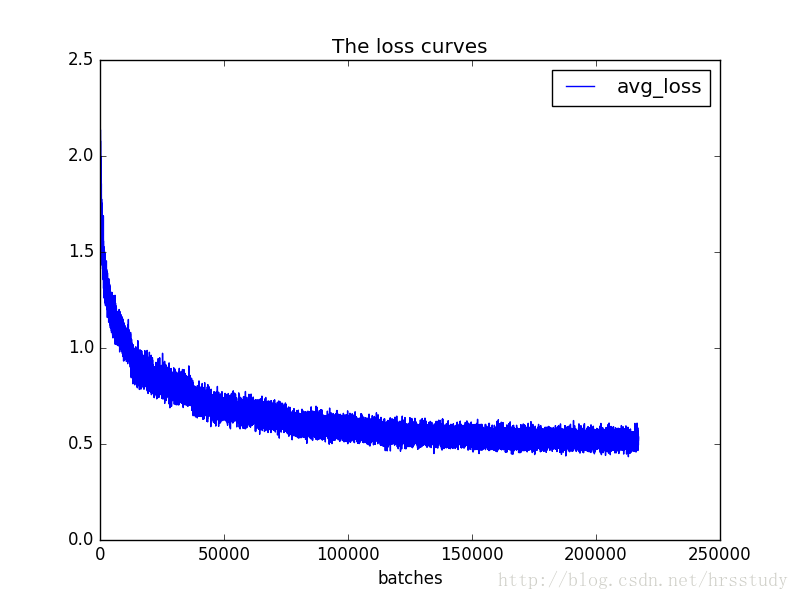
\includegraphics[scale=0.6]{figures/curve_loss.png}
%\caption{DeepFlow Training accuracy}
%\label{deepFlow_graph}
%\end{figure}

\newpage
\begin{figure}
\centering
\begin{subfigure}{.5\textwidth}
  \centering
  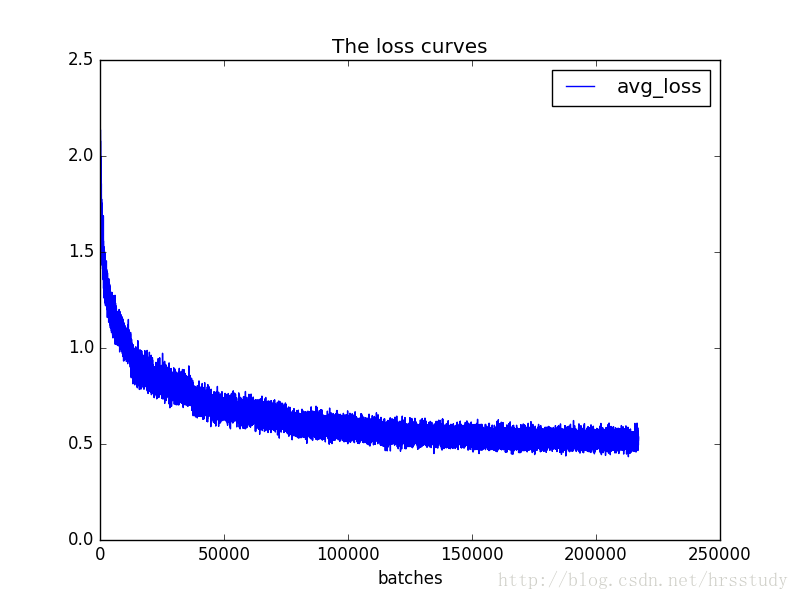
\includegraphics[width=.5\linewidth]{figures/curve_loss.png}
  \caption{DeepFlow Training accuracy}
  \label{fig:deepFlow_graph}
\end{subfigure}%
\begin{subfigure}{.5\textwidth}
  \centering
  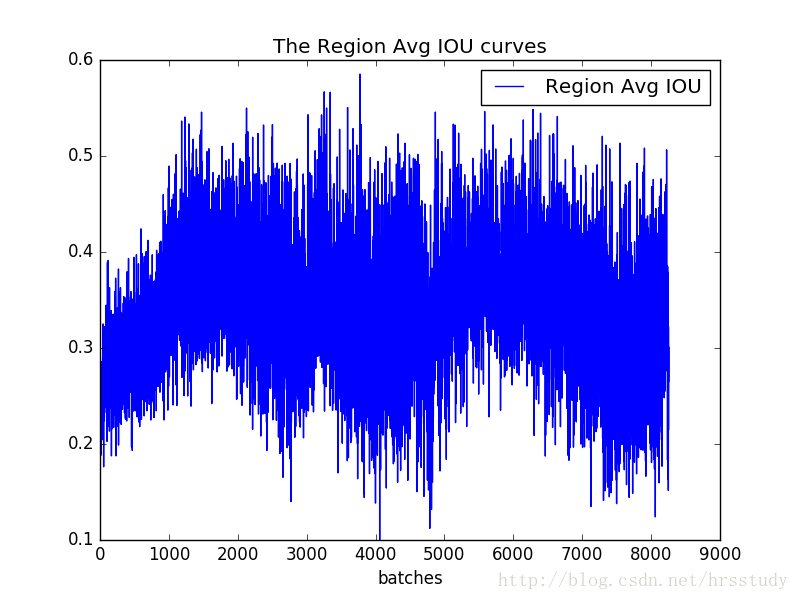
\includegraphics[width=.5\linewidth]{figures/avg_IOU.png}
  \caption{DeepFlow IOU}
  \label{fig:DeepFlow_IOU}
\end{subfigure}
\caption{DeepFlow Object Detection Accuracy Test}
\label{fig:deep_accuracy}
\end{figure}

From the loss curve  in figure \ref{deep_accuracy} \ref{deepFlow_graph}, it can be seen that while training our model again the decline rate of the loss function is very slow, almost no decline, when it reaches a certain number of iterations. Further analysis of the log and .cfg files reveals that the custom learning rate change strategy, we set, is reduced by ten times over 100,000 iterations resulting in a decrease in loss rate. Therefore, we perform some modifications on the learning rate change strategy in cfg to get better results.

To further improve DeepFlow, we had to also optimize the IOU (figure \ref{IOU_fig}) obtained during or training. IOU is a great way to determine how accurate our model is able to perform detection of certain objects.If we get a 100\% IOU, we would have a perfect detection system: a perfect overlap of our bounding box and the target. 

\begin{figure}[ht]
\centering
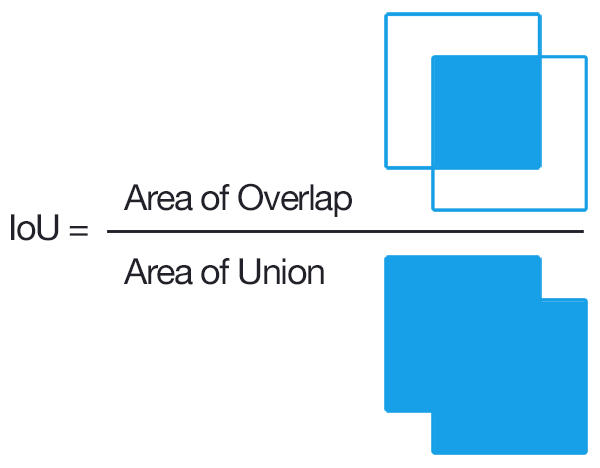
\includegraphics[scale=0.2]{figures/IOU.png}
\caption{DeepFlow IOU}
\label{IOU_fig}
\end{figure}

The test image above shows how really the model is learning, where it becomes easier to detect objects in monochrome backgrounds (like airplanes into the figure of the
whole process), but training to detect generalized object, where this condition is not satisfied, gives us a lower accuracy, more if overlapped object are present.

\begin{figure}
\centering
\begin{subfigure}{.4\textwidth}
  \centering
  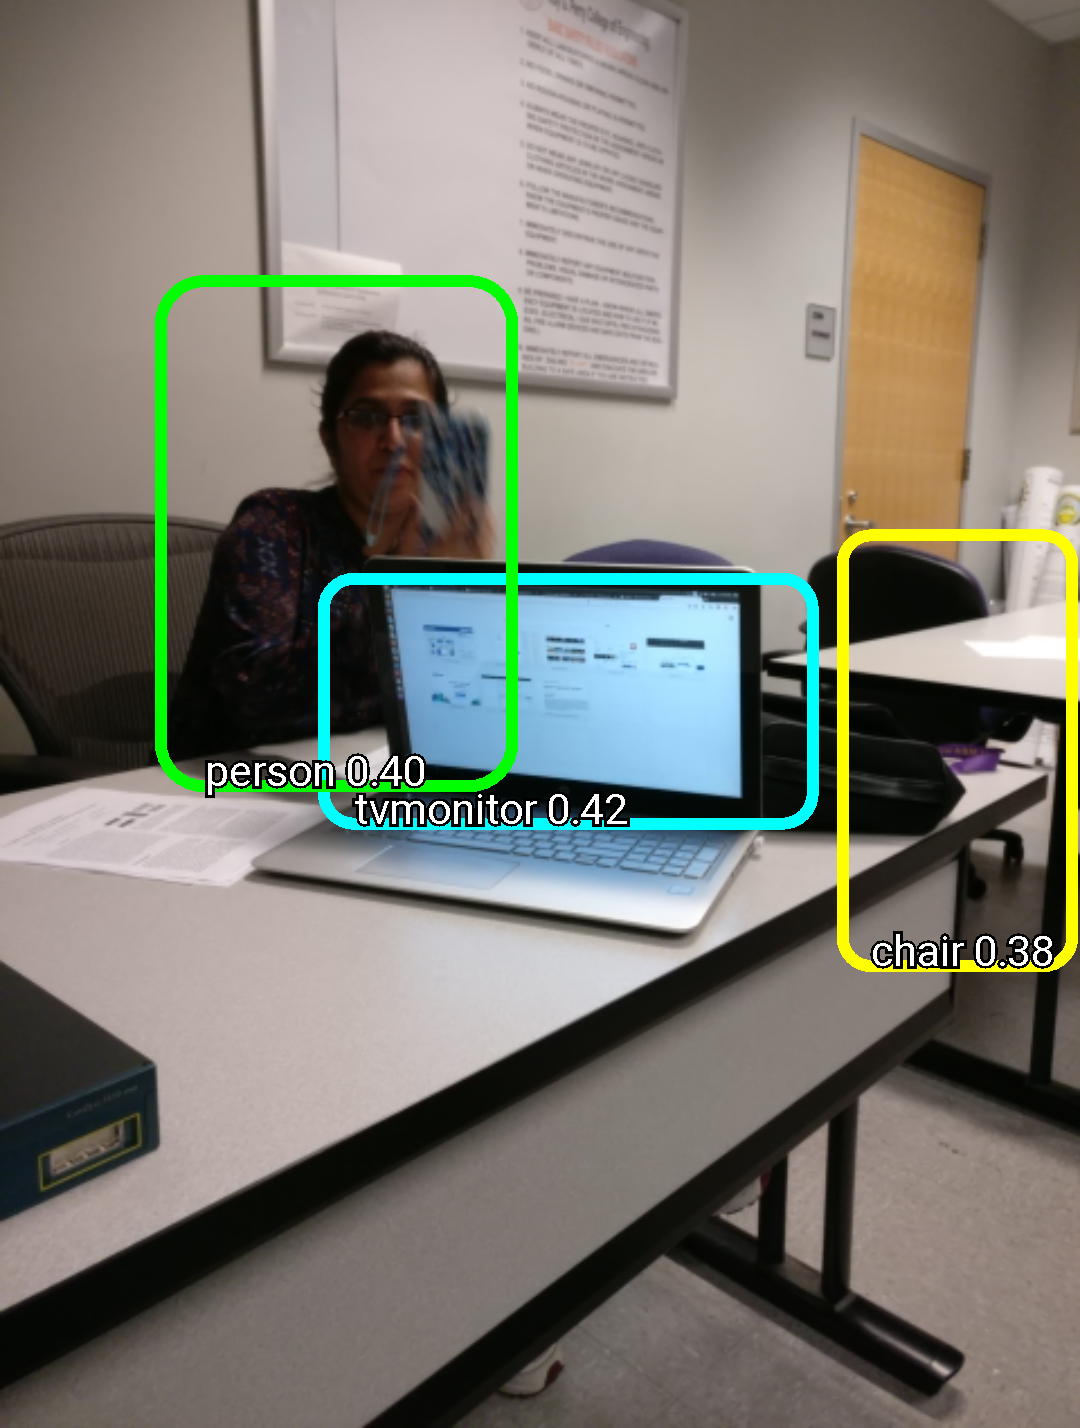
\includegraphics[width=.5\linewidth]{figures/test_4.png}
  \caption{DeepFlow Test}
  \label{fig:deepFlow_graph}
\end{subfigure}
\begin{subfigure}{.4\textwidth}
  \centering
  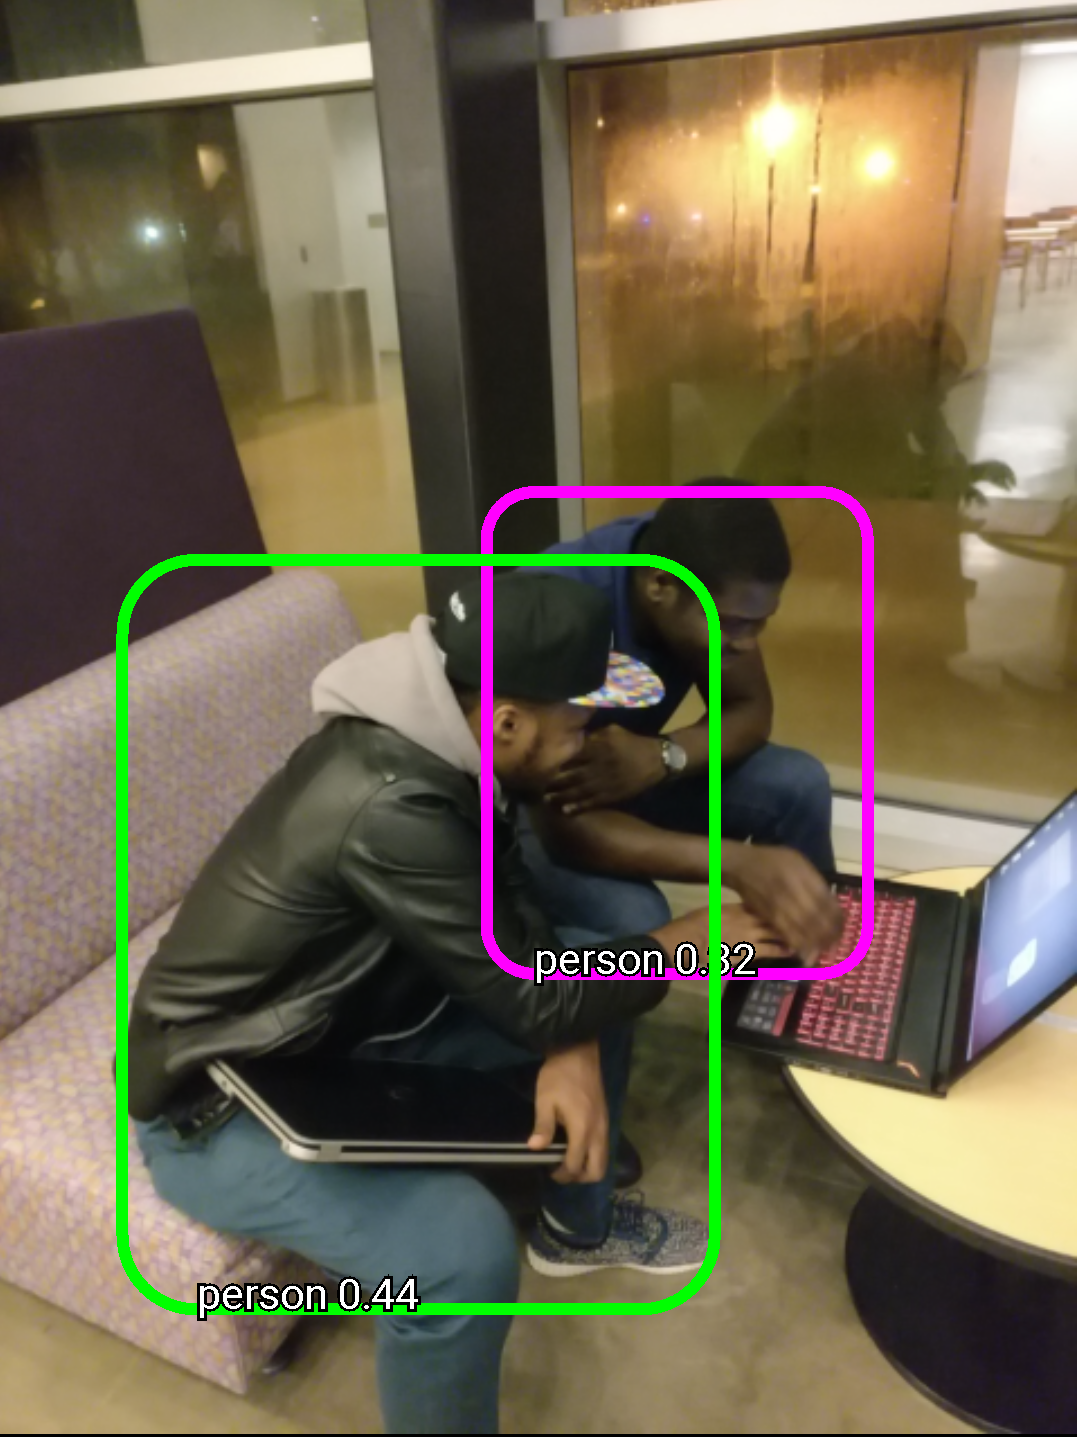
\includegraphics[width=.5\linewidth]{figures/test_1.png}
  \caption{DeepFlow IOU}
  \label{fig:DeepFlow_IOU}
\end{subfigure}
\begin{subfigure}{.4\textwidth}
  \centering
  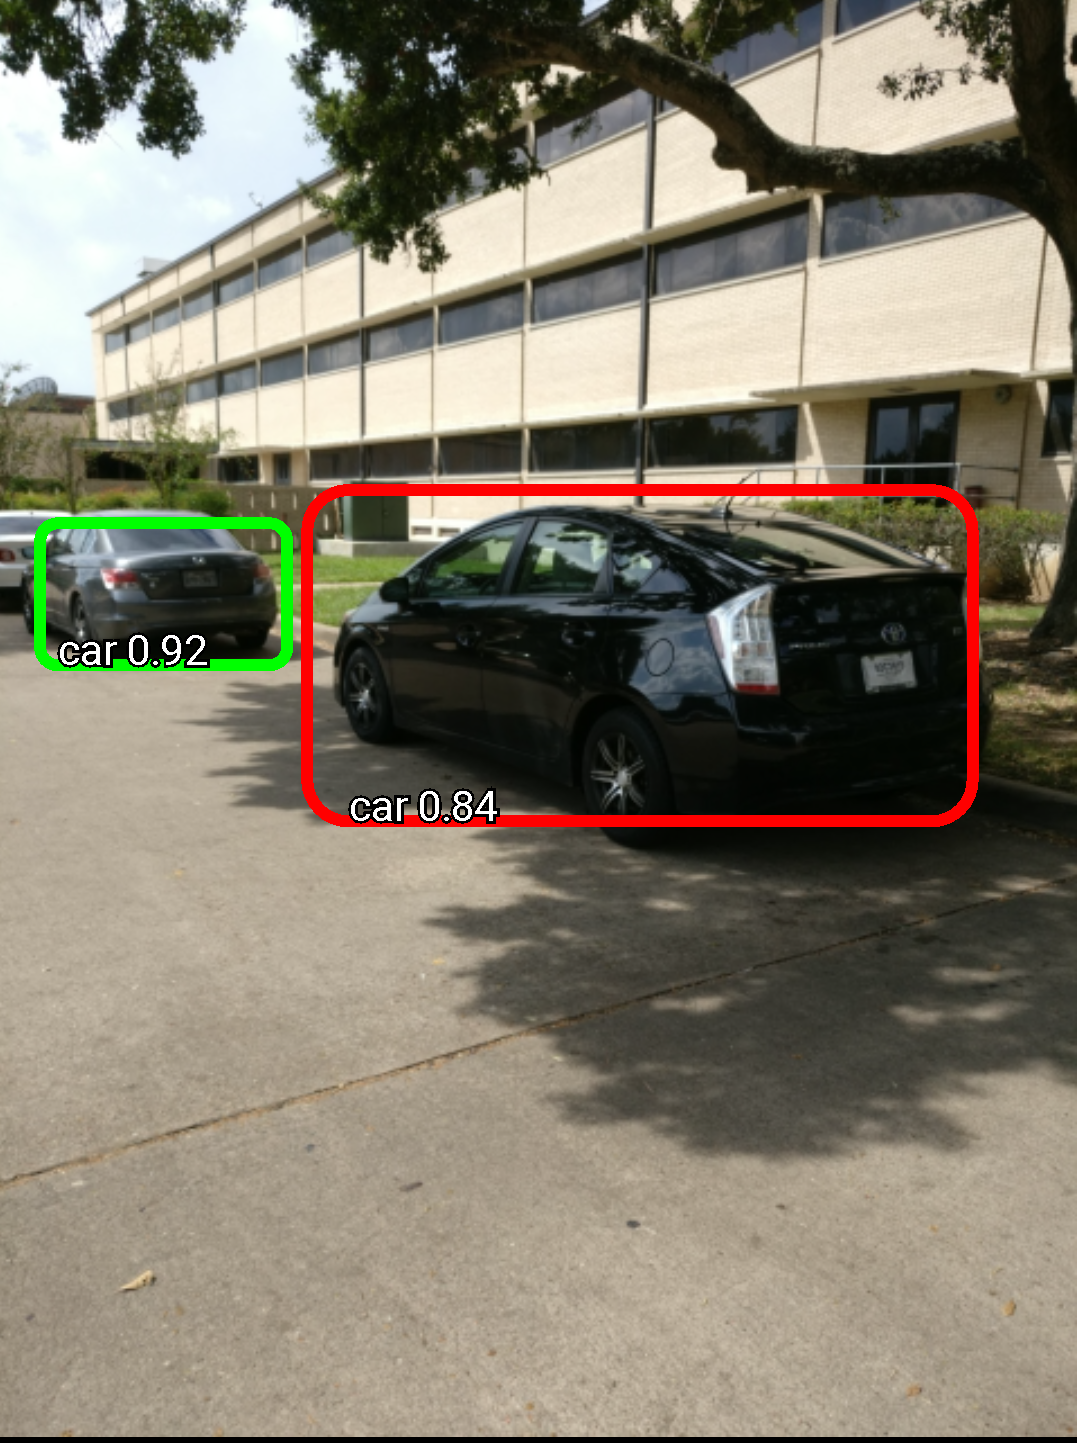
\includegraphics[width=.5\linewidth]{figures/test_3.png}
  \caption{DeepFlow  Test}
  \label{fig:deepFlow_graph}
\end{subfigure}
\begin{subfigure}{.4\textwidth}
  \centering
  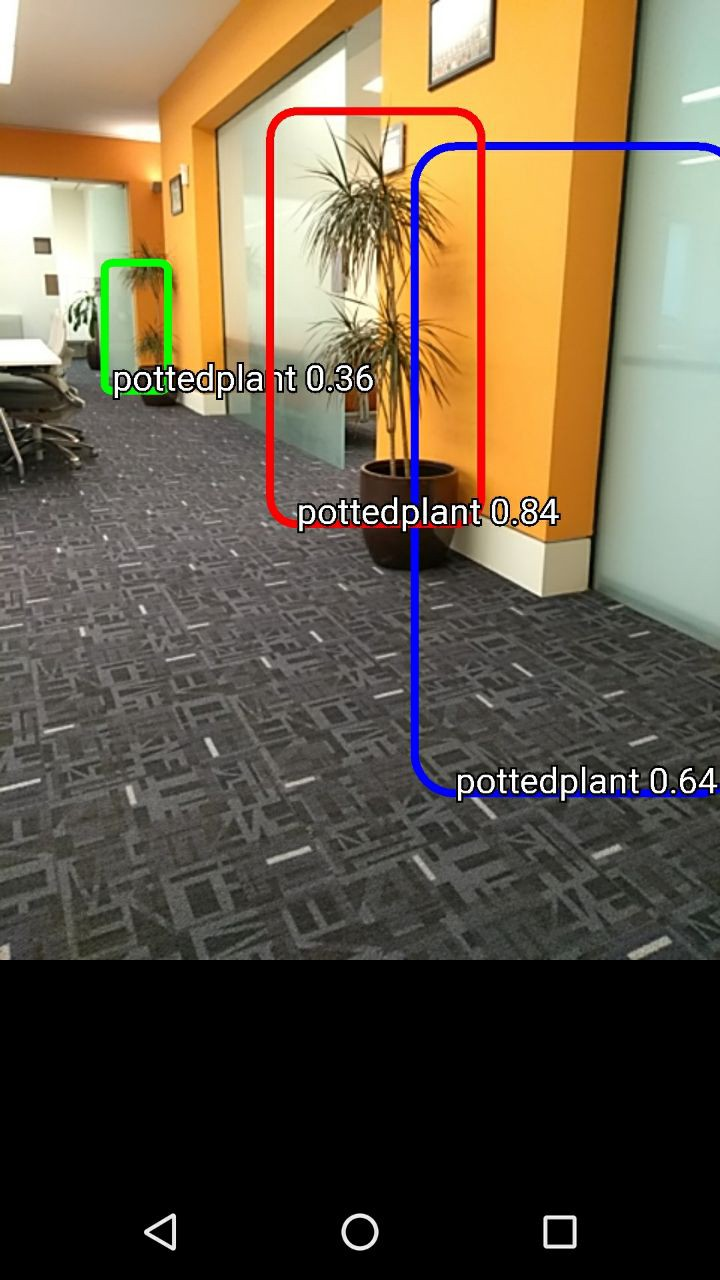
\includegraphics[width=.5\linewidth]{figures/test_6.jpeg}
  \caption{DeepFlow IOU}
  \label{fig:DeepFlow_IOU}
\end{subfigure}
\caption{DeepFlow  Test}
\label{fig:deep_accuracy}
\end{figure}

%\begin{figure}
%\centering
%\begin{subfigure}{.4\textwidth}
%  \centering
%  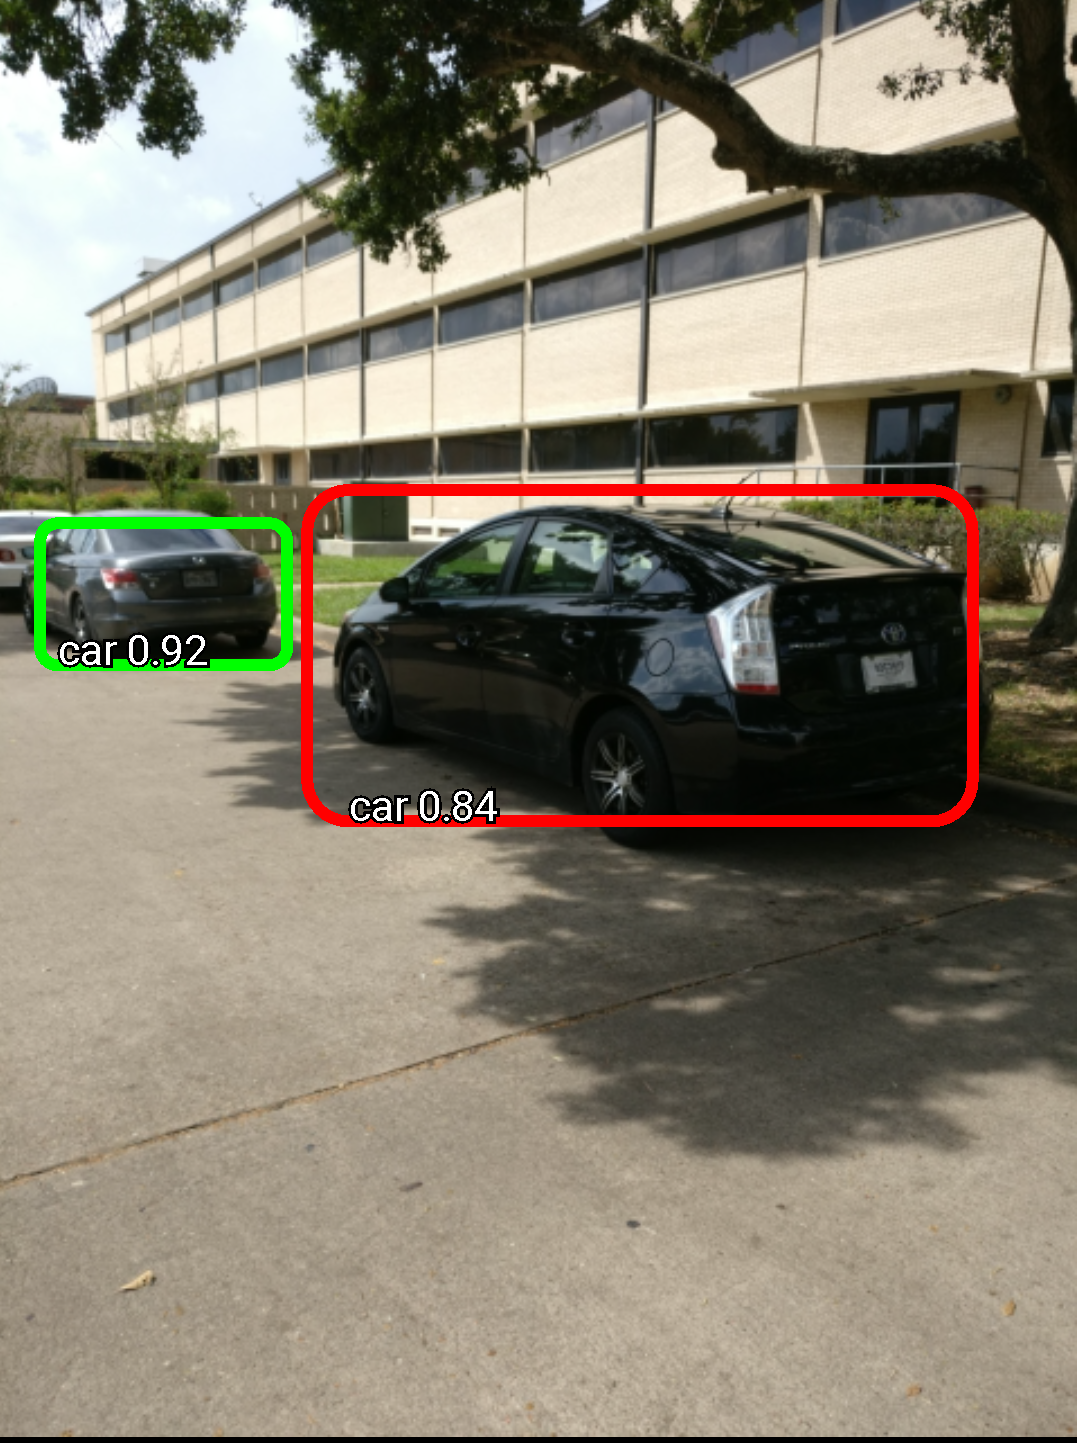
\includegraphics[width=.5\linewidth]{figures/test_3.png}
%  \caption{DeepFlow  Test}
%  \label{fig:deepFlow_graph}
%\end{subfigure}%
%\begin{subfigure}{.4\textwidth}
%  \centering
%  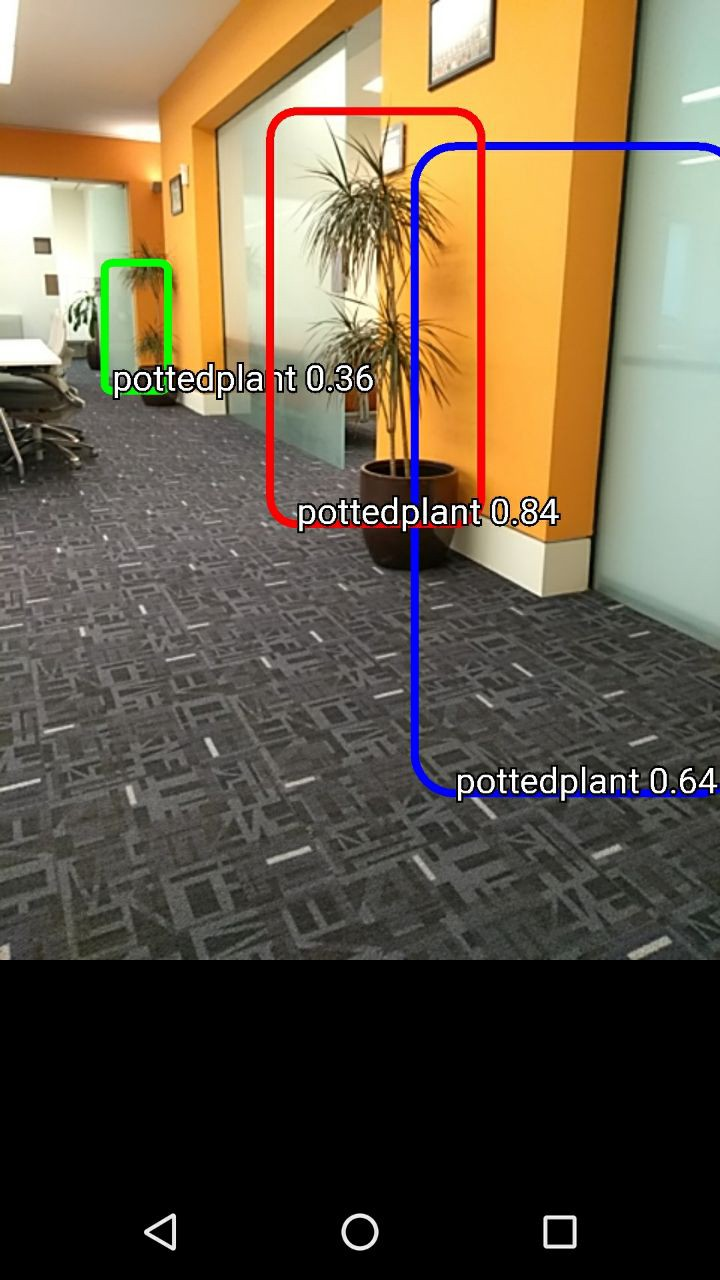
\includegraphics[width=.5\linewidth]{figures/test_6.jpeg}
%  \caption{DeepFlow IOU}
%  \label{fig:DeepFlow_IOU}
%\end{subfigure}
%\caption{DeepFlow Test}
%\label{fig:deep_accuracy}
%\end{figure}

\section{Object Detection Test}

To evaluate how effective is our algorithm in terms of its detection ability, a standard test was set up. We place different objects at specific distances from the drone’s onboard camera to calculate and record the number of seconds in which an object has been detected when there has been movement. We also calculate the number of seconds that the object has not been detected because movement has not been detected, and the seconds in which the algorithm has detected an object as false positive.  For the calculation of the seconds a cell phone stop watch has been used and it has been calculated approximately the seconds in which the algorithm does not detect the object or gives a false positive with human supervision, these data will therefore be totally approximated taking into account the error caused by human visual perception (0.2s). These last times have also been calculated with timer and has taken into account the treatment of experimental errors using the following formulas:

\begin{itemize}
	\item $ Arithmetic  Mean  = \overline{x} =  {\frac{\sum_{i=1}^{n} x_i }{n}} $ 
	\item $ Standard  Deviation  =  \sigma =  {\sqrt{\frac{n}{n -1}*{(\bar{x} - {x_i})^2}}} $ 
	\item $ Accidental  Error  = \varepsilon{_{acc}} =  {\frac{\sigma}{\sqrt{n}}} $ 	
	\item $ Instrument  Error  = \varepsilon{_{ins}} =  {0.01s} $ 	
	\item $ Human  Error  = \varepsilon{_{hum}} =  {0.02s} $ 	
	\item $ Total  Error  = \varepsilon{_{tot}}=  {\sqrt{e_{acc}^{2} + e_{ins}^{2}}} $ 		 
\end{itemize}

\section{Test 1}
The first test for detecting objects was made at a distance of 1m. The result is shown in the image itself by trimming the region representing the zone that is detected. The results obtained are shown in the following table in figure \ref{object_table_1}:

\begin{figure}[ht]
\centering
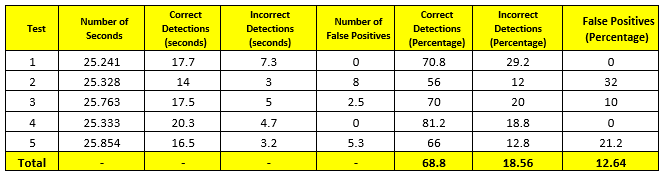
\includegraphics[scale=0.8]{figures/test_table_1.png}
\caption{Object Detection test 1}
\label{object_table_1}
\end{figure}

\pagebreak
\begin{itemize}
	\item $ \overline{x} = \frac{25.241 +  25.328 + 25.763  + 25.333 +  25.854} {5} = \frac{127.519}{5} = 25.504s $ 	
	\item $ \sigma =  {\sqrt{\frac{(25.241 - 25.504)^2 +  (25.328 - 25.504)^2 + (25.763 - 25.504)^2  + (25.333 - 25.504)^2+  (25.854 - 25.504)^2}{5 - 1}}} = 0.282s$
	\item $\varepsilon{_{acc}} =  {\frac{0.282}{\sqrt{5}}} = 0.126s$
	\item $\varepsilon{_{tot}}=  {\sqrt{0.126^{2} + 0.01^{2}}} = 0.126s$
	\item $ \varepsilon{_{ins}} =  {0.01s} $ 	
\end{itemize}

In this test, we have taken samples every \begin{math}25.000\pm0.126s\end{math}. With the algorithm of detecting objects by movement in 1m we see that it is able to detect the object that is being moved in question with a success of 68.8\%. The calculation of time with motion detection is very approximate since it is complicated to process the pixel differences continuously and sometimes false positives \begin{math}(0.3\pm0.2 s)\end{math} and \begin{math}(0.4\pm0.2 s)\end{math} by the movement itself the drone.


\section{Test 2}
The second test of detecting objects was carried out at a distance of 3m. with the same conditions that were already mentioned previously. The results obtained are shown in the table of figure \ref{object_table_2} below:

\begin{figure}[ht]
\centering
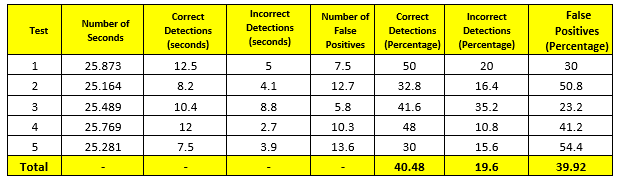
\includegraphics[scale=0.8]{figures/test_table_2.png}
\caption{Object Detection test 2}
\label{object_table_2}
\end{figure}

\pagebreak
\begin{itemize}
	\item $ \overline{x} = \frac{25.873 +  25.164 + 25.489  + 25.769 +  25.281} {5} = \frac{127.576}{5} = 25.515s $ 	
	\item $ \sigma =  {\sqrt{\frac{(25.873 - 25.515)^2 +  (25.164 - 25.515)^2 + (25.489 - 25.515)^2  + (25.769 - 25.515)^2+  (25.281 - 25.515)^2}{5 - 1}}} = 0.305s$
 	\item $\varepsilon{_{acc}} =  {\frac{0.305}{\sqrt{5}}} = 0.136s$
	\item $\varepsilon{_{tot}}=  {\sqrt{ 0.305s^{2} + 0.01^{2}}} = 0.136s$
	\item $ \varepsilon{_{ins}} =  {0.01s} $ 	
\end{itemize}

In this test, we have taken samples every \begin{math}25.000\pm0.136s\end{math}. The results are very similar to those of the previous test. In this case the probability of success is 40.48\% and the false positives were produced with approximate times of \begin{math} 0.3\pm0.2s\end{math}.


\section{Test 3}
The third test was carried out at a distance of 4m. under the same conditions that were mentioned previously. The results obtained are shown in the figure \ref{object_table_3} of the table below:

\begin{figure}[h]
\centering
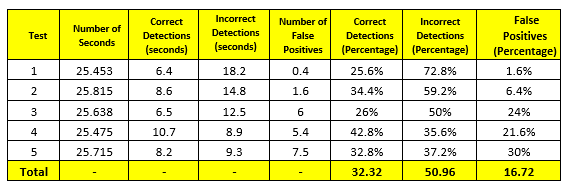
\includegraphics[scale=0.8]{figures/test_table_3.png}
\caption{Object Detection test 3}
\label{object_table_3}
\end{figure}

\pagebreak
\begin{itemize}
	\item $ \overline{x} = \frac{25.453 +  25.815 + 25.638  + 25.475 + 25.715} {5} = \frac{126.595}{5} = 25.319s $ 	
	\item $ \sigma =  {\sqrt{\frac{(25.453 - 25.319)^2 +  (25.815 - 25.319)^2 + (25.638 - 25.319)^2  + (25.475 - 25.319)^2+  ( 25.715 - 25.319)^2}{5 - 1}}} = 0.449s$
	\item $\varepsilon{_{acc}} =  {\frac{0.449}{\sqrt{5}}} = 0.201s$
	\item $ \varepsilon{_{ins}} =  {0.01s} $ 
\end{itemize}

In this test, we have taken samples every \begin{math}25.000\pm0.225 s.\end{math} With a distance of 4m. the detection test gets worse results than the previous ones. This is because the drone having a greater distance, the connection loses intensity and sometimes more temporal lapses occur. In addition, by having more field of view, the algorithm detects the most pixelated object so it is more difficult to find the characteristics of the object. Several temporal lapses of approximately \begin{math}0.3\pm0.2 s\end{math}, \begin{math}0.2\pm0.2 s\end{math} and \begin{math}0.8\pm0.2 s\end{math} occur. In this case, we obtain a 32.32\% success that is still an acceptable percentage and therefore continues to provide reliability to the algorithm.


\section{Recognition test}

\section{Test 1}
The first test for object recognition was made by placing a bottle in front of the camera and gradually move it. The image has been classified with three different distances of 1m, 3m and 4m. The result is displayed in a ranking of 5 probabilities where the object being viewed is classified. The results obtained are reflected in the table in figure \ref{classification_table} below: 


\begin{figure}[ht]
\centering
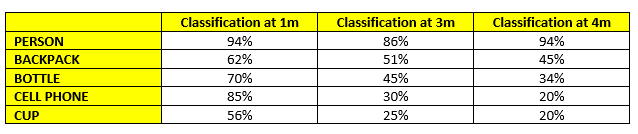
\includegraphics[scale=0.8]{figures/recognition_table_1.png}
\caption{Classification results at difference distances}
\label{classification_table}
\end{figure}

Since the object recognition did not depend strictly on the algorithms, the results were obtained in order to know the optimal distance to obtain data coherent with the classification of the API of the neural network. If we analyze the total results obtained, we see that it has the capacity to obtain valid results for objects that are at a distance of 1 to 6 meters, although with really low probability (uncertainty). For objects that are at a distance of 7 meters or more, the results are very low, but always providing a response. In addition, it should be noted that the recognition API returned very exact results in terms of the type of object. In terms of moving images, the results are not so good at times because the captures are produced with a very fine blurry layer (due to movement) which provides some inaccurate results.


\section{Tracking Test}

The objective in this test is to get the drone to move with the object that is being detected so that the maneuvers follow the following flight pattern:

\begin{enumerate}
\item Raise the flight
\item Detect object.
\item Stay stable for a few seconds.
\item Move the object so that the drone follows an upward movement.
\item Move the object so that the drone follows a downward movement.
\item Move the object so that the drone follows a movement to the right.
\item Move the object so that the drone follows a leftward movement.
\item Follow a circular motion surrounding the drone so that it can perform a 360-degree turn.
\item Land.
\end{enumerate}

We must be aware to see when the drone performs any of the actions correctly in a timed period of time and will be marked as done or not. The time will stop the moment the drone completes the route, stops responding to the commands or loses the connection.

\section{Test 1}
The first test of tracking was done moving a bottle in front of the drone’s onboard camera with the parameters that are reflected in Table 3.40. The values of Amin and Amax have been defined from the most optimal distance (1.5 - 3m) that allows the drone to detect the object more easily and allow it to center the object in the middle of the camera.

\begin{figure}[ht]
\centering
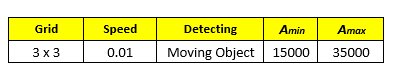
\includegraphics[scale=0.8]{figures/tracking_test_settings_1.png}
\caption{tracking test setup}
\label{tracking_test_setup}
\end{figure}

The results obtained are shown in firgure \ref{} in Table below. To better understand the behavior, a box has been defined per table in which the number of the action to be performed is displayed and whether it has been executed correctly or not.

\begin{figure}[ht]
\centering
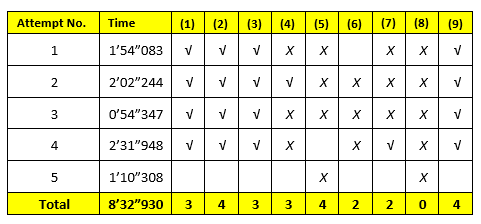
\includegraphics[scale=0.8]{figures/tracking_test_results_1.png}
\caption{tracking test results}
\label{tracking_test_results_1}
\end{figure}

from the table above, we can see that:

\begin{itemize}
\item Attempt No. 1: Does not correctly detect the object being moved. Detects several false positives.
\item Attempt No. 2: It begins to detect the moving object, but the kinetic itself makes it lose stability.
\item Attempt No. 3: Same as the second attempt.
\item Attempt No. 4: Same as the first attempt.
\item Attempt No. 5: Same as the first attempt.
\end{itemize}

\section{Test 2}

The second test of tracking was carried out with the parameters that are reflected in Table in figure \ref{tracking_test_setup}:

\begin{figure}[ht]
\centering
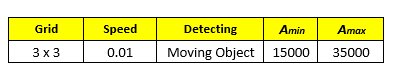
\includegraphics[scale=0.8]{figures/tracking_test_settings_1.png}
\caption{tracking test setup}
\label{tracking_test_setup}
\end{figure}

Results are shown in the the figure \ref{tracking_test_results_2} of the table below:

\begin{figure}[ht]
\centering
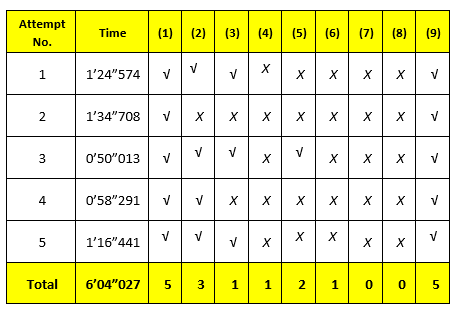
\includegraphics[scale=0.8]{figures/tracking_test_results_2.png}
\caption{tracking test results}
\label{tracking_test_results_2}
\end{figure}

Results are very similar to the first attempt for which as a future work commands sent to drone have to be improved as we detect and track objects:

\begin{itemize}
\item Attempt No. 1: When it detects the object, it doesn’t move. Even though, the algorithm is actually tracking.
\item Attempt No. 2: It does not detect the object and many false positives occur.
\item Attempt No. 3: Similar to the first attempt. False positives cause the object to not move properly.
\item Attempt No. 4: Does not correctly detect the object. It loses connection and therefore stability.
\item Attempt No. 5: We can detect Object Motions clearly but drone doesn’t move.
\end{itemize}

In general, when tracking detection problems persist. Most false positives occur because the camera picks up its own motions and confuses the plane. In the tracking method, we see that the results are not optimal and that it is not possible to perform almost any actions, due to the false positives of the cinematic movement of the drone and its own stabilizer. In addition, the tests were shorter because it suffered continually due to the heaviness and the delay of the algorithm itself.

